\subsection{Triangular Factorization}

\frame{
\begin{itemize}
\item In the above section, we saw how easy it is to solve an upper-triangular system. 
\vspace{3mm}
\item Now we introduce the concept of factorization of a given matrix $A$ into the product of a lower triangular matrix $L$ that has 1`s along the main diagonal and an upper-triangular matrix $U$ with nonzero diagonal elements. 
\vspace{3mm}
\item For ease of notation we illustrate the concepts with matrices of dimension $4 \times 4$, but they apply to an arbitrary system of dimension $N \times N$. 
\end{itemize}
}

\frame{
\begin{block}{Definition.}
The nonsingular matrix $A$ has a {\Large triangular factorization} if it can be expressed as the product of a lower-triangular matrix $L$ and an upper-triangular matrix $U$
\begin{equation*}
A = L U
\end{equation*}
In matrix form, this is written as
\begin{equation*}
\left[
\begin{array}{c c c c}
a_{1,1} & a_{1,2} & a_{1,3} & a_{1,4} \\
a_{2,1} & a_{2,2} & a_{2,3} & a_{2,4} \\
a_{3,1} & a_{3,2} & a_{3,3} & a_{3,4} \\
a_{4,1} & a_{4,2} & a_{4,3} & a_{4,4} 
\end{array}
\right]
=
\left[
\begin{array}{c c c c}
1 & 0 & 0 & 0\\
m_{2,1} & 1 & 0 & 0\\
m_{3,1} & m_{3,2} & 1 & 0\\
 m_{4,1} & m_{4,2} & m_{4,3} & 1
\end{array}
\right]
\left[
\begin{array}{c c c c}
u_{1,1} & u_{1,2} & u_{1,3} & u_{1,4} \\
0 & u_{2,2} & u_{2,3} & u_{2,4} \\
0 & 0 & u_{3,3} & u_{3,4} \\
0 & 0 & 0 & u_{4,4} 
\end{array}
\right]
\end{equation*}
The condition that $A$ is nonsingular implies that $u_{k,k} \ne 0$ for all $k$. 
The notation for the entries in $L$ is $m_{i,j}$.
%and the reason for the choice of $m_{i,j}$ instead of $l_{i,j}$ will be pointed out soon.
\end{block}
}


\frame{
\frametitle{Solution of a Linear System}
Suppose that the coefficient matrix $A$ for the linear system $AX = B$ has a triangular factorization; 
then the solution to
\begin{equation*}
L U X = B
\end{equation*}
can be obtained by defining $Y = U X$ and then solving two systems:
\begin{itemize}
\item first solve $LY = B$ for $Y$
\item then solve $UX = Y$ for $X$
\end{itemize}
}

\frame{
In equation form, we must first solve the lower-triangular system
\begin{equation*}
\begin{array}{r c r c r c r c c}
y_1 & & & & & & & = & b_1 \\
m_{2,1}y_1 & + & y_2 & & & & & = & b_2 \\
m_{3,1}y_1 & + & m_{3,2}y_2 & + & y_3 & & & = & b_2 \\
m_{4,1}y_1 & + & m_{4,2}y_2 & + & m_{4,3}y_3 & + & y_4 & = & b_2
\end{array}
\end{equation*}
to obtain $y_1$, $y_2$, $y_3$, and $y_4$ and use them in solving the upper-triangular system
\begin{equation*}
\begin{array}{r c r c r c r c c}
u_{1,1}x_1 & + & u_{1,2}x_2 & + & u_{1,3}x_3 & + & u_{1,4}x_4 & = & y_1 \\
& & u_{2,2}x_2 & + & u_{2,3}x_3 & + & u_{2,4}x_4 & = & y_2 \\
& & & & u_{3,3}x_3 & + & u_{3,4}x_4 & = & y_3 \\
& & & & & & u_{4,4}x_4 & = & y_4
\end{array}
\end{equation*}
}


\frame{
\frametitle{Example }
Solve
\begin{equation*}
\begin{array}{r c r c r c r c r}
x_1   & + & 2x_2 & + & 4x_3 & + & x_4   & = & 21 \\
2x_1 & + & 8x_2 & + & 6x_3 & + & 4x_4 & = & 52 \\
3x_1 & + & 10x_2 & + & 8x_3 & + & 8x_4 & = & 79 \\
4x_1 & + & 12x_2 & + & 10x_3 & + & 6x_4 & = & 82
\end{array}
\end{equation*}
\begin{center}
$\Downarrow$
\end{center}
Use the triangular factorization method and the fact that
\begin{equation*}
A = 
\left[
\begin{array}{l l l l}
1 & 2 & 4 & 1 \\
2 & 8 & 6 & 4 \\
3 & 10 & 8 & 8 \\
4 & 12 & 10 & 6
\end{array}
\right]
= 
\left[
\begin{array}{l l l l}
1 & 0 & 0 & 0 \\
2 & 1 & 0 & 0 \\
3 & 1 & 1 & 0 \\
4 & 1 & 2 & 1
\end{array}
\right]
\left[
\begin{array}{l l l l}
1 & 2 & 4 & 1 \\
0 & 4 & -2 & 2 \\
0 & 0 & -2 & 3 \\
0 & 0 & 0 &-6
\end{array}
\right]
= L U 
\end{equation*}
}

\frame{
Use the forward-substitution method to solve $LY = B$
\begin{equation*}
\begin{array}{r c r c r c r c  r}
y_1   &    &        &     &         &      &      & = & 21 \\
2y_1 & + & y_2 &     &         &      &      & = & 52 \\
3y_1 & + & y_2 & + &   y_3 &     &       & = & 79 \\
4y_1 & + & y_2 & + & 2y_3 & + & y_4 & = & 82
\end{array}
\end{equation*}
\begin{center}
$\Downarrow$
\end{center}
Compute the values 
\begin{itemize}
\item $y_1 = 21$
\item $y_2 = 52 - 2(21) = 10$
\item $y_3 = 79 - 3(21) - 10 = 6$
\item $y_4 = 82 - 4(21) - 10 - 2(6) = -24$, 
\end{itemize}
or 
\begin{equation*}
Y = \left[ \begin{array}{c c c c}
21 & 10 & 6 & -24
\end{array} \right]^{T}
\end{equation*}
}

\frame{
Next write the system $U X = Y$
\begin{equation*}
\begin{array}{r c r c r c r c  l}
x_1 & + & 2x_2 & + &  4x_3  & + &    x_4 & = & 21 \\
       &    & 4x_2 & - &  2x_3  & + &   2x_4 & = & 10 \\
       &    &         &     & -2x_3 & + &   3x_4 & = & 6 \\
       &     &        &     &            &     & -6x_4 & = & -24
\end{array}
\end{equation*}
\begin{center}
$\Downarrow$
\end{center}
Now use {\Large back substitution} and compute the solution 
\begin{itemize}
\item $x_4 = -24/(-6) = 4$
\item $x_3 = (6 - 3(4))/(-2) = 3$
\item $x_2 = (10 - 2(4) + 2(3))/4 = 2$
\item $x_1 = 21 - 4 - 4(3) - 2(2) = 1$ 
\end{itemize}
or
\begin{equation*}
X = \left[ \begin{array}{c c c c}
1 & 2 & 3 & 4
\end{array} \right]^{T}
\end{equation*}
}



\frame{
\frametitle{Triangular Factorization}
\begin{block}{}
If row interchanges are not necessary when using Gaussian elimination, the multipliers $m_{ij}$ are the subdiagonal entries in $L$. 
\end{block}
Example: \\
Use Gaussian elimination to construct the triangular factorization of the matrix
\begin{equation*}
A = 
\left[
\begin{array}{r r r}
4    &   3 & -1 \\
-2 & -4 &   5 \\
1    &   2 &   6
\end{array}
\right]
\end{equation*}
The matrix $L$ will be constructed from an identity matrix placed at the left.  \\
For each row operation used to construct the upper-triangular matrix, the multipliers $m_{i,j}$ will be put in their proper places at the left.
}

\frame{
Start with 
\begin{equation*}
A = 
\left[
\begin{array}{r r r}
1 & 0 & 0 \\
0 & 1 & 0 \\
0 & 0 &  1
\end{array}
\right]
\left[
\begin{array}{r r r}
4    &   3 & -1 \\
-2 & -4 &   5 \\
1    &   2 &   6
\end{array}
\right]
\end{equation*}
\begin{center}
$\Downarrow$
\end{center}
Row $1$ is used to eliminate the elements of $A$ in column $1$ below $a_{1,1}$.  \\
The multiples $m_{2,1} = -0.5$ and $m_{3,1} = 0.25$ of row $1$ are subtracted from rows $2$ and $3$, respectively.  \\
\begin{center}
$\Downarrow$
\end{center}
These multipliers are put in the matrix at the left and the result is
\begin{equation*}
A = 
\left[
\begin{array}{r r r}
1 & 0 & 0 \\
-0.5 & 1 & 0 \\
0.25 & 0 &  1
\end{array}
\right]
\left[
\begin{array}{r r r}
4 &   3      & -1 \\
0 & -2.5  &   4.5 \\
0 &   1.25 &   6.25
\end{array}
\right]
\end{equation*}
}

\frame{
\begin{center}
$\Downarrow$
\end{center}
\begin{itemize}
\item Row $2$ is used to eliminate the elements in column $2$ below the diagonal of the second factor of $A$ in the above product. 
\item The multiple $m_{3,2} = -0.5$ of the second row is subtracted from row $3$, and the multiplier is entered in the matrix at the left and we have the desired triangular factorization of $A$.
\end{itemize}
\begin{equation*}
A = 
\left[
\begin{array}{r r r}
1 & 0 & 0 \\
-0.5 & 1 & 0 \\
0.25 & -0.5 &  1
\end{array}
\right]
\left[
\begin{array}{r r r}
4 &   3      & -1 \\
0 & -2.5  &   4.5 \\
0 &   0     &   8.5
\end{array}
\right]
\end{equation*}
}

\frame{
\begin{block}{Theorem (Direct Factorization $A = LU$ : No Row Interchanges).} 
Suppose that Gaussian elimination, without row interchanges, can be performed successfully to solve the general linear system $AX = B$. 
Then the matrix $A$ can be factored as the product of a lower-triangular matrix $L$ and an upper-triangular matrix $U$:
\begin{equation*}
A = L U
\end{equation*}
Furthermore, $L$ can be constructed to have $1’s$ on its diagonal and $U$ will have nonzero diagonal elements. 
After finding $L$ and $U$, the solution $X$ is computed in two steps:
\begin{itemize}
\item Solve $LY = B$ for $Y$ using forward substitution.
\item Solve $UX = Y$ for $X$ using back substitution.
\end{itemize}
\end{block}
}

\frame{
\frametitle{Proof of Theorem}
When the Gaussian elimination process is followed and $B$ is stored in column $N+1$ of the augmented matrix, the result after the uppertriangularization step is the equivalent upper-triangular system $UX = Y$. \\
}

\frame{
The matrices $L$, $U$, $B$, and $Y$ will have the form
\begin{equation*}
L = 
\left[
\begin{array}{c c c c c}
1 & 0 & 0 & \cdots & 0 \\
m_{2,1} & 1 & 0 & \cdots & 0 \\
m_{3,1} & m_{3,2} & 1 & \cdots & 0 \\
\vdots & \vdots & \vdots & & \vdots \\
m_{N,1} & m_{N,2} & m_{N,3} & \cdots & 1
\end{array}
\right], 
%\end{equation*}
%\begin{equation*}
B =
\left[
\begin{array}{ c }
a^{(1)}_{1, N+1} \\
a^{(2)}_{2, N+1} \\
a^{(3)}_{3, N+1} \\
\vdots \\
a^{(N)}_{N, N+1}
\end{array}
\right]
\end{equation*}

\begin{equation*}
U =
\left[
\begin{array}{c c c c c}
a^{(1)}_{1,1} & a^{(1)}_{1,2} & a^{(1)}_{1,3} & \cdots a^{(1)}_{1,N} \\
0 & a^{(2)}_{2,2} & a^{(2)}_{2,3} & \cdots & a^{(2)}_{2,N} \\
0 & 0 & a^{(3)}_{3,3} & \cdots & a^{(3)}_{3,N} \\
\vdots & \vdots & \vdots & & \vdots \\
0 & 0 & 0 & \cdots & a^{(N)}_{N,N}
\end{array}
\right], 
Y =
\left[
\begin{array}{ c }
a^{(1)}_{1, N+1} \\
a^{(2)}_{2, N+1} \\
a^{(3)}_{3, N+1} \\
\vdots \\
a^{(N)}_{N, N+1}
\end{array}
\right]
\end{equation*}
\begin{block}{Remark.}
To find just $L$ and $U$, the $(N + 1)$st column is not needed.
\end{block}
}

\frame{
Step 1. \\
Store the coefficients in the augmented matrix.  \\
The superscript on $a^{(1)}_{r,c}$ means that this is the first time that a number is stored in location $(r, c)$.
\begin{equation*}
\left[
\begin{array}{c c c c c | c}
a_{1,1}^{(1)} & a_{1,2}^{(1)} & a_{1,3}^{(1)} & \cdots & a_{1,N}^{(1)} & a_{1,N+1}^{(1)} \\
a_{2,1}^{(1)} & a_{2,2}^{(1)} & a_{2,3}^{(1)} & \cdots & a_{2,N}^{(1)} & a_{2,N+1}^{(1)}\\
a_{3,1}^{(1)} & a_{3,2}^{(1)} & a_{3,3}^{(1)} & \cdots & a_{3,N}^{(1)} & a_{3,N+1}^{(1)}\\
\vdots        & \vdots        & \vdots        &            & \vdots             & \vdots \\
a_{N,1}^{(1)} & a_{N,2}^{(1)} & a_{N,3}^{(1)} & \cdots & a_{N,N}^{(1)} & a_{N,N+1}^{(1)}
\end{array}
\right]
\end{equation*}
}

\frame{
Step $2$ 	.
Eliminate $x_1$ in rows $2$ through $N$ and store the multiplier $m_{r,1}$, used to eliminate $x_1$ in row $r$, 
in the matrix at location $(r, 1)$.
\begin{figure}
\begin{center}
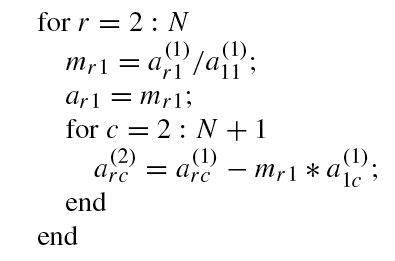
\includegraphics[width=35mm]{chap-2/P145_Step2.png}
\end{center}
\end{figure}
The new elements are written $a^{(2)}_{r,c}$ to indicate that this is the second time that a number has been stored in the matrix at location $(r, c)$.  \\
The result after step 2 is
\begin{equation*}
\left[
\begin{array}{c c c c c | c}
a_{1,1}^{(1)} & a_{1,2}^{(1)} & a_{1,3}^{(1)} & \cdots & a_{1,N}^{(1)} & a_{1,N+1}^{(1)} \\
m_{2,1}        & a_{2,2}^{(2)} & a_{2,3}^{(2)} & \cdots & a_{2,N}^{(2)} & a_{2,N+1}^{(2)}\\
m_{3,1}       & a_{3,2}^{(2)} & a_{3,3}^{(2)} & \cdots & a_{3,N}^{(2)} & a_{3,N+1}^{(2)}\\
\vdots        & \vdots        & \vdots        &            & \vdots             & \vdots \\
m_{N,1}       & a_{N,2}^{(2)} & a_{N,3}^{(2)} & \cdots & a_{N,N}^{(2)} & a_{N,N+1}^{(2)}
\end{array}
\right]
\end{equation*}
}

\frame{
Step $3$.
Eliminate $x_2$ in rows $3$ through $N$ and store the multiplier $m_{r,2}$, used to eliminate $x_2$ in row $r$ , in the matrix at location $(r, 2)$.
\begin{figure}
\begin{center}
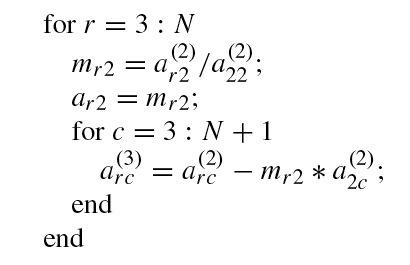
\includegraphics[width=35mm]{chap-2/P145_Step3.png}
\end{center}
\end{figure}
The new elements are written $a^{(3)}_{r,c}$ to indicate that this is the third time that a number has been stored in the matrix at the location $(r, c)$.
\begin{equation*}
\left[
\begin{array}{c c c c c | c}
a_{1,1}^{(1)} & a_{1,2}^{(1)} & a_{1,3}^{(1)} & \cdots & a_{1,N}^{(1)} & a_{1,N+1}^{(1)} \\
m_{2,1}        & a_{2,2}^{(2)} & a_{2,3}^{(2)} & \cdots & a_{2,N}^{(2)} & a_{2,N+1}^{(2)}\\
m_{3,1}       & m_{3,2}         & a_{3,3}^{(3)} & \cdots & a_{3,N}^{(3)} & a_{3,N+1}^{(3)}\\
\vdots        & \vdots        & \vdots        &            & \vdots             & \vdots \\
m_{N,1}       & m_{N,2}      & a_{N,3}^{(3)} & \cdots & a_{N,N}^{(3)} & a_{N,N+1}^{(3)}
\end{array}
\right]
\end{equation*}
}

\frame{
Step $p + 1$\footnote{This is the general step}. 
Eliminate $x_p$ in rows $p + 1$ through $N$ and store the multipliers at the location $(r, p)$.
\begin{figure}
\begin{center}
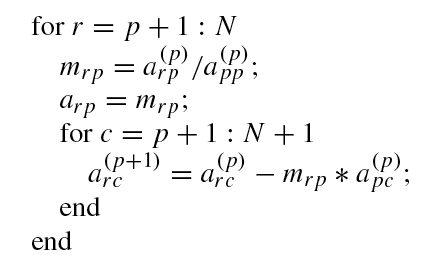
\includegraphics[width=35mm]{chap-2/P146_StepP.png}
\end{center}
\end{figure}
The final result after $x_{N-1}$ has been eliminated from row $N$ is
\begin{equation*}
\left[
\begin{array}{c c c c c | c}
a_{1,1}^{(1)} & a_{1,2}^{(1)} & a_{1,3}^{(1)} & \cdots & a_{1,N}^{(1)} & a_{1,N+1}^{(1)} \\
m_{2,1}        & a_{2,2}^{(2)} & a_{2,3}^{(2)} & \cdots & a_{2,N}^{(2)} & a_{2,N+1}^{(2)}\\
m_{3,1}       & m_{3,2}         & a_{3,3}^{(3)} & \cdots & a_{3,N}^{(3)} & a_{3,N+1}^{(3)}\\
\vdots        & \vdots        & \vdots        &            & \vdots             & \vdots \\
m_{N,1}       & m_{N,2}      & m_{N,3}        & \cdots & a_{N,N}^{(N)} & a_{N,N+1}^{(N)}
\end{array}
\right]
\end{equation*}
}

\frame{
We must now verify that the product $LU = A$.  \\
Suppose that $D = LU$ and consider the case when $r \le c$. 
Then $d_{r,c}$ is
\begin{equation*}
d_{r,c} = m_{r,1} a^{(1)}_{1,c} + m_{r,2} a^{(2)}_{2, c} + \cdots + m_{r,r-1}a^{(r-1)}_{r-1,c} + a^{(r)}_{r,c}
\end{equation*}
Using the replacement equations in steps $1$ through $p+1 = r$ , we obtain the following substitutions:
\begin{equation*}
\begin{array}{r c l}
m_{r,1} a^{(1)}_{1,c} & = & a^{(1)}_{r,c} - a^{(2)}_{r, c}, \\
m_{r,2} a^{(2)}_{2,c} & = & a^{(2)}_{r,c} - a^{(3)}_{r,c}, \\
& \vdots & \\
m_{r,r-1} a^{(r-1)}_{r-1,c} & = & a^{(r-1)}_{r,c} - a^{(r)}_{r,c}.
\end{array}
\end{equation*}
\begin{center}
$\Downarrow$
\end{center}
\begin{equation*}
d_{r,c} =  a^{(1)}_{r,c}  - a^{(2)}_{r, c} + a^{(2)}_{r, c} - a^{(3)}_{r, c} + \cdots + a^{(r-1)}_{r,c} - a^{(r)}_{r,c} + a^{(r)}_{r,c} = a^{(1)}_{r,c}
\end{equation*}
The other case, $r > c$, is similar to prove.
}


\frame{
\frametitle{Computational Complexity}
\begin{itemize}
\item The process for triangularizing is the same for both the Gaussian elimination and triangular  factorization methods. 
\vspace{2mm}
\item We can count the operations if we look at the first $N$ columns of the augmented matrix in Theorem 2.6. 
\vspace{2mm}
\item The outer loop of step $p + 1$ requires $N - p = N - (p + 1) + 1$ divisions to compute the multipliers $m_{rp}$.
\vspace{2mm}
\item Inside the loops, but for the first $N$ columns only, a total of $(N - p)(N - p)$ multiplications and  the same number of subtractions are required to compute the new row elements $a_{rc}^{(p+1)}$ . 
\vspace{2mm}
\item This process is carried out for $p = 1,2, ... ,N - 1$. 
\end{itemize}
}

\frame{
The triangular factorization portion of $A = LU$ requires
\begin{equation*}
\sum_{p=1}^{N-1} (N-p)(N-p+1) = \frac{N^3 - N}{3} \ \ multiplications \ \ and \ \ divisions
\end{equation*}
and
\begin{equation*}
\sum_{p=1}^{N-1} (N-p)(N-p) = \frac{2N^3 - 3N^2 + N}{6} \ \ subtractions.
\end{equation*}
To establish the above equation, we use the summation formulas
\begin{equation*}
\sum_{k=1}^{M} k = \frac{M(M+1)}{2}
\end{equation*}
and
\begin{equation*}
\sum_{k=1}^{M} k^2 = \frac{M(M+1)(2M+1)}{6}
\end{equation*}
}

\frame{
\begin{itemize}
\item Once the triangular factorization $A=L U$ has been obtained, the solution to the lower-triangular system $LY=B$ will require $0 + 1 + ... + N - 1 = (N2 - N)\slash2$ multiplications and subtractions; no divisions are required because the diagonal elements of $L$ are 1's. 
\item Then the solution of the upper-triangular system $UX = Y$ requires $1 + 2 + ... + N = (N2 + N)\slash2$ multiplications and divisions and $(N2 - N)\slash2$ subtractions. 
\item Therefore, finding the solution to $LUX =B$ requires 
\end{itemize}
\begin{block}{}
{\huge $N^2$ multiplications and divisions,\\ and $N^2 - N$ subtractions.}
\end{block}
}

\frame{
\begin{itemize}
\item We see that the bulk of the calculations lies in the triangularization portion of the solution. 
\vspace{2mm}
\item If the linear system is to be solved many times, with the same coefficient matrix $A$ but with different column matrices $B$, it is not necessary to triangularize the matrix each time if the factors are saved. 
\vspace{2mm}
\item This is the reason the triangular factorization method is usually chosen over the elimination method. 
\vspace{2mm}
\item However, if only one linear system is solved, the two methods are the same, except that the triangular factorization method stores the multipliers. 
\end{itemize}
}


